

\section{Definitionen und Technologie}
\label{sec:definitionen-und-technologie}

In dieser Sektion werden die Grundlegenden Technologie und Definitionen beschrieben die zum Verständnis von autonomen Fahren wichtig sind.

\subsection{SAE-Level}
\label{ssec:sae-level}

Die SAE-Level \cite{standardSAE} beschreiben den Grad an Autonomie bei autonomen Fahrzeugen. Sie werden dabei in 6 unterschiedliche Stufen unterschieden und wurden von der \citeauthor{standardSAE} definiert.\\

\subsubsection*{Level 0 - Keine Automatisierung} Der Fahrer übernimmt die volle Kontrolle über das Fahrzeug.

\subsubsection*{Level 1 - Fahrassistenz} Der Fahrer wird durch einen einzelnen Fahrassistenten, z.B. Tempomat, Spurhalteassistent oder Bremsassistent, unterstützt, behält jedoch die volle Kontrolle über das Fahrzeug.

\subsubsection*{Level 2 - Partielle Automatisierung} Der Fahrer wird durch mehrere Fahrassistenten unterstützt and hat immer die Kontrolle über das Fahrzeug.
    
\subsubsection*{Level 3 - Bedingte Automatisierung} Das Fahrzeug ist in der Lage die Umgebung zu erkennen und ist in der Lage eigenständig in bestimmten Fahrsituationen zu meistern. Ein aufmerksamer Fahrer ist noch erforderlich, der unter Umständen einschreiten kann.

\subsubsection*{Level 4 - Hohe Automatisierung} Das Fahrzeug ist in der Lage sich eigenständig in den meisten Fahrumgebungen zu manövrieren. Es erkennt Fehlentscheidungen und kann auf diese reagieren. Menschliches einschreiten ist, wenn gewünscht, möglich.

\subsubsection*{Level 5 - Volle Automatisierung} Das Fahrzeug kann in allen Umgebungen und zu jederzeit und in jeder Situation komplett eigenständig Fahren.

\subsection{Sensoren}

In Autonomen Fahrzeugen kommen unterschiedliche Arten von Sensoren zum Einsatz. 
Dazu gehören Kameras, Radars, spezielle Laserscanner und Ultraschallsensoren.\\

\begin{figure}[H]
    \centering
    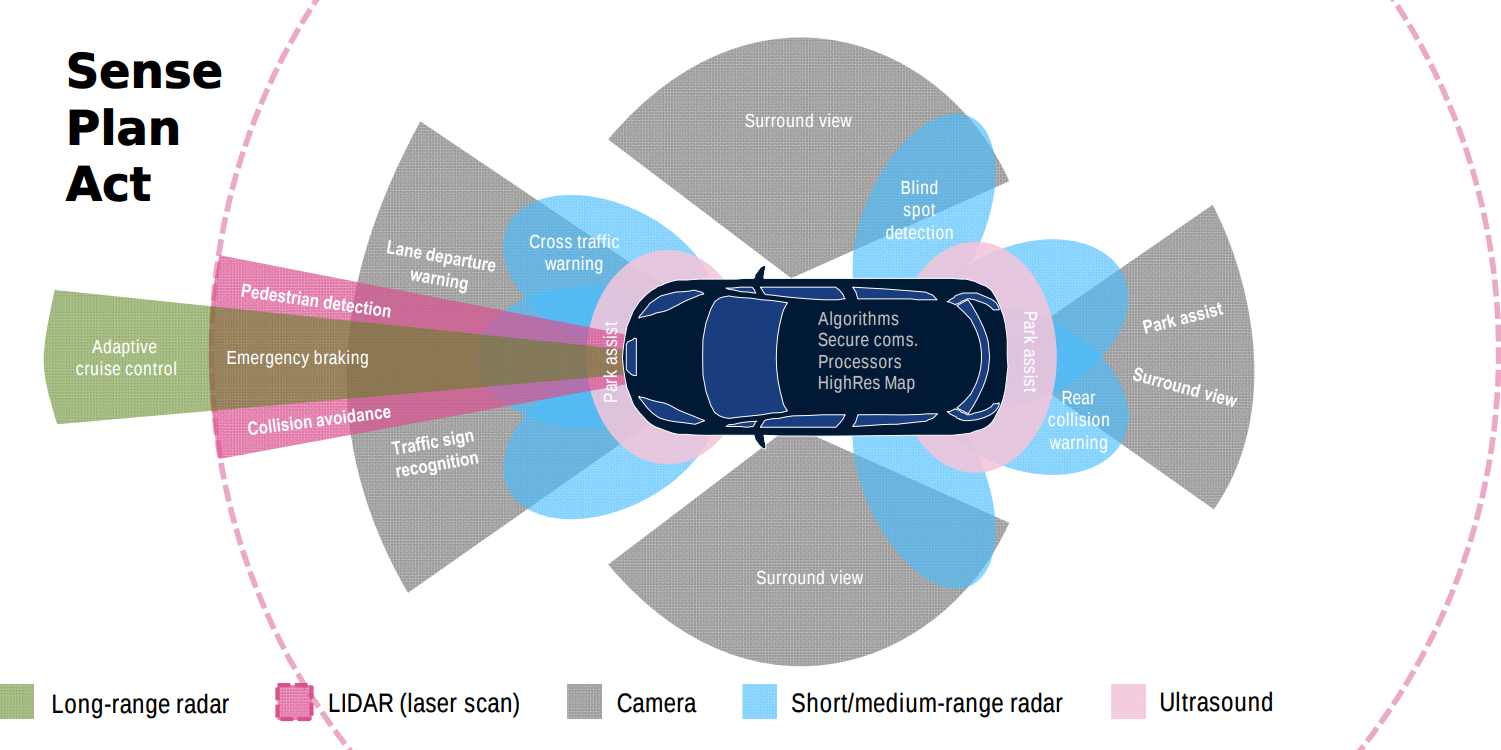
\includegraphics[width=.485\textwidth]{resources/images/sensors.png}
    \caption{Sensoren eines autonomen Fahrzeuges \cite{smith2015automated}}
\end{figure}

Kameras können rund um das Fahrzeug montiert werden und ermöglichen dem Fahrzeug somit eine vollumfängliche Sicht auf das Verkehrsgeschehen. Ein Vorteil gegenüber einem menschlichen Fahrer ist, das auch tote Winkel mit Kameras überwacht werden können. Lediglich durch die geschossenen Bilder der Kameras lässt sich jedoch die Entfernung zu erkannten Objekten schlecht einschätzen.\\

Hier kommt die LIDAR-Technologie \cite{himmelsbach2008lidar} ins Spiel. LIDAR steht für \textit{Light Detection and Ranging}. Es handelt sich um eine Umgebungsüberwachungstechnik die mit Hilfe eines Lasers Objekte in der Nähe bestrahlt und die Reflexion mit einem Sensor misst. So kann die Entfernung zu den Objekten berechnet werden.\\

Radar-Systeme \cite{introductionToRadarSystems} funktionieren ähnlich wie LIDAR-Systeme. Anstatt von Lichtwellen werden Radiowellen eingesetzt. Objekte in der Umgebung erzeugen ein Echo, welches vom einem Sensor empfangen wird. Somit ist ein Radar-System in der Lage die Distanz, Position und Geschwindigkeit von Objekten zu berechnen.\\

Neben Radar- und LIDAR-Systemen können weitere Sensoren in autonomen Fahrzeugen zum Einsatz kommen. Hierzu zählen beispielsweise Ultraschall und Infrarot.
Ultraschall wird auch in der Natur von Fledermäusen eingesetzt. Es funktioniert ähnlich wie ein Radar, hat jedoch eine geringere Reichweite und ist somit besser geeignet um Objekte in der direkten Umgebung des Fahrzeuges zu erkennen.\\

Mit Hilfe der verschiedenen Sensorsystemen, ist man in der Lage ein komplettes 3D-Abbild der Umgebung zu erstellen. Durch den Einsatz von Radar können selbst Objekte die sich hinter anderen Objekten, und somit mit rein optischen Sensoren nicht zu erkennen wären, entdeckt werden. Damit hat ein autonomes Fahrzeug einen entscheidenden Vorteil gegenüber einem Menschen, der Objekte außerhalb seines Sichtfeldes nicht identifizieren kann.\\

\subsection{Vehicular Ad-hoc Network}

Fahrzeuge vernetzen sich mit anderen Fahrzeugen und der Infrastruktur über ein \textit{VANET}. Das \textit{VANET} ist eine Abwandlung des \textit{MANETs (Mobile Ad-hoc Network)}. 

\begin{figure}[H]
    \centering
    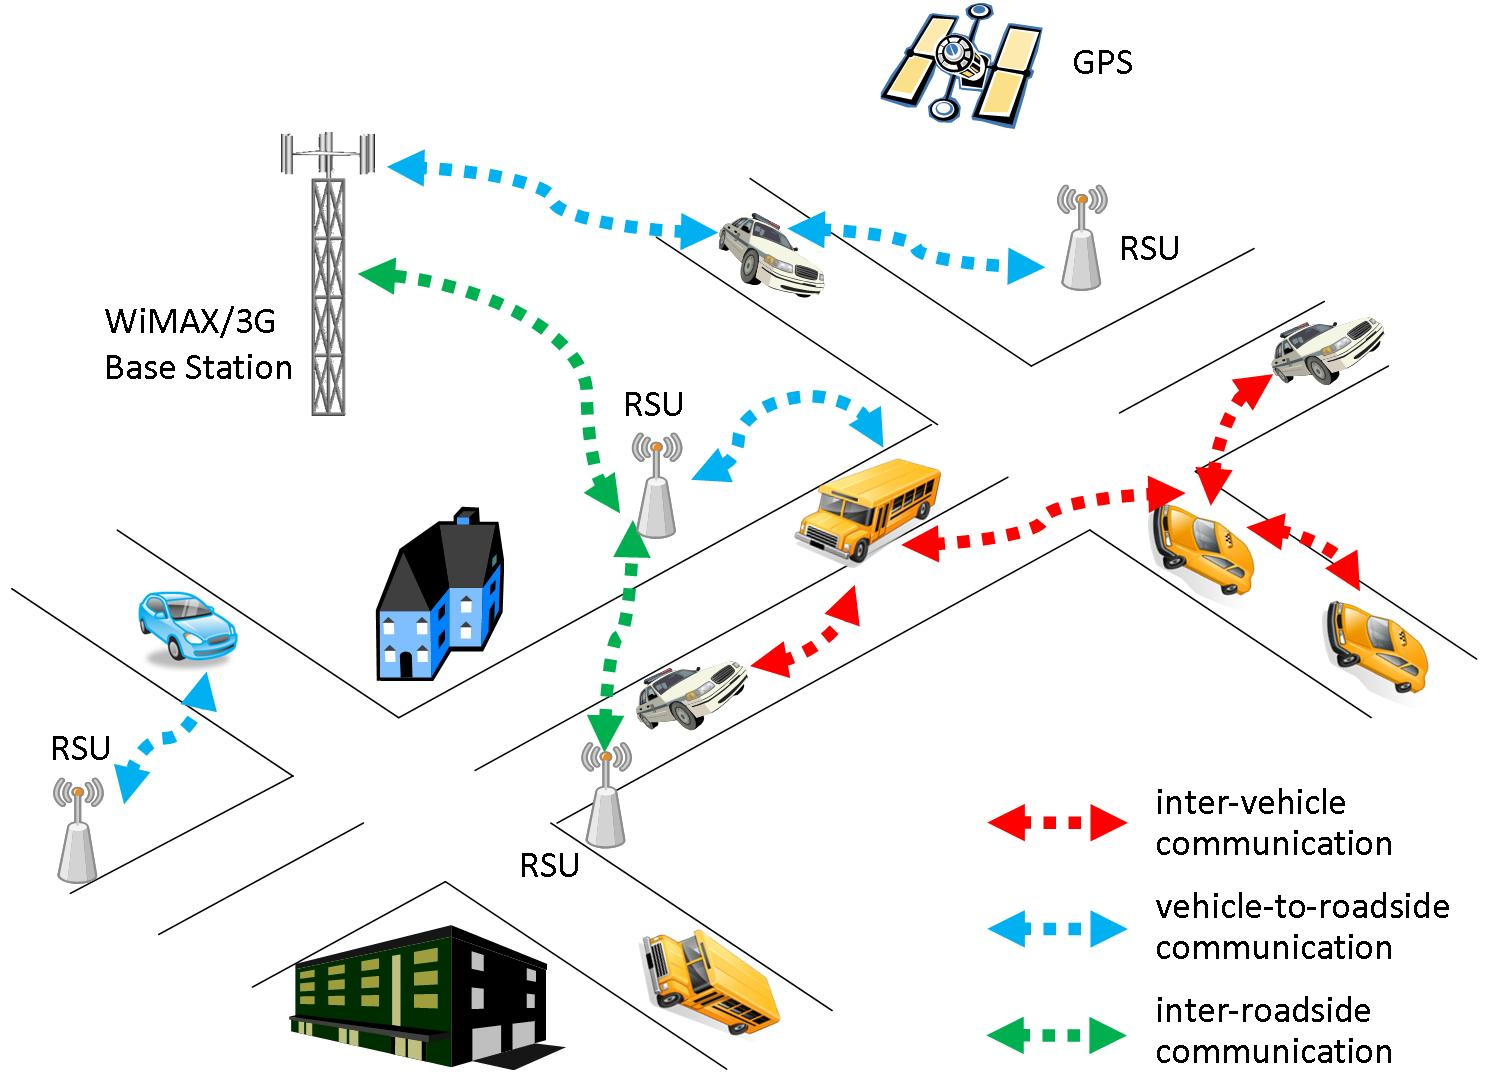
\includegraphics[width=.485\textwidth]{resources/images/vanet.jpg}
    \caption{Übersichtsgrafik eines VANETs \cite{vanet}}
\end{figure}

Durch die Verwendung von VANETs sind Fahrzeuge in der Lage untereinander und mit der Infrastruktur zu kommunizieren. Somit kann eine Ampel ihren aktuellen Status an das passierende Fahrzeug senden und Ihm mitteilen ob Sie Rot, Gelb oder Grün leuchtet. Das Fahrzeug kann darauf hin eine Entscheidung Treffen wie es sich verhalten soll. Eine weitere Anwendungsmöglichkeit ist beispielsweise die Stauerkennung. Fahrzeuge können untereinander kommunizieren ob Sie sich in einem Stau befinden. So können andere Verkehrsteilnehmer gewarnt werden und entsprechende Stauabschnitte automatisch Umfahren werden.

\subsection{Software}

In autonomen Fahrzeugen kommt unterschiedliche Software zum Einsatz. Algorithmen aggregieren die Daten der Sensoren und treffen Entscheidungen über den Fahrtverlauf. Außerdem übernimmt Software die Kommunikation zu anderen Verkehrsteilnehmer und der Infrastruktur. Damit sich die Fahrzeuge besser orientieren können werden hochauflösende Karten eingesetzt.